\chapter{Background}\label{background}
%----------------------------------------------------------------
%
% Traffic Generator
%
%----------------------------------------------------------------
\section{Traffic Generator}\label{sec:tg}
The more the \gls{it} infrastructures and networks grow, the higher the demand there is to test and validate its behavior as more devices connect.
The network providers and researchers use traffic generator tools to a large extent for experiments, performance testing, verification and validation~\cite{botta2010you, molnar2013validate}.
As pointed out in the recent studies the network testing tools are either software- or hardware-based platforms~\cite{turull2016pktgen, emmerich2015moongen, antichi2014osnt, ghobadi2012caliper}.

\subsection{Why Software-Based Traffic Generator}
The network research community commonly uses or develops, open-source and software-based networking tools.
In contrast, network equipment and solution providers often use proprietary and hardware-based ones, for example, Spirent~\cite{Networkd93:online} and Ixia~\cite{IxiaMake81:online}.
These are proprietary and specialized software and hardware for network testing.
Flexibility, accuracy, and cost are the factors for this general division between hardware- and software-based platforms.
That is, 1) software-based networking tools are more flexible and cheaper than the hardware-based platform, on the other hand, 2) hardware-based tools generate more accurate and realistic network traffic than software-based tools at higher rates.

\skippara \citet*{botta2010you} identified that the flexibility of software-based network tools narrows down to three points.
First, the ease to deploy these tools in a distributed fashion.
Second, the freedom to make changes to fit a specific research purpose.
Third, it can run on top of a variety of \glspl{os} and its networking stack.
However, a hardware-based platform is more rigor and stable for network testing, because of its specialization.

\skippara The traffic's accuracy comes down to how well a network provider can fulfill the customer's requirements, for example, a mobile operator or an \gls{isp}.
These profiles are often rigor and detailed data sheets that describe, for example, a specified speed or correctness within an error interval.
Software-based tools often do not meet these requirements.
That is, without knowledge of underlying hardware and software, there is a high chance to produce inaccurate results.
Thus, \citet*{botta2010you} examined four software traffic generators and tried to raise awareness within the network research community to assess traffic generators critically.

\subsection{Metrics and Types}\label{metrictype}
There is a vast amount of software-based traffic generators with different purposes, for example, \cite{DITGDist48:online, Packetge32:online, ToolsThe22:online} are three lists of traffic generators to only mention a few.
Therefore, \citet{botta2010you, molnar2013validate} have attempted to categorize most frequently used traffic generators in the papers ``Do you trust your software-based traffic generator'' and ``How to validate traffic generators?'' respectively.
Both found that the most frequently used traffic generators in literature are packet-level and maximum throughput traffic generators, which we marked with an asterisk in \cref{types}.
Moreover, conventional metrics are byte throughput, packet size, and inter-departure/packet time distribution.

\begin{table}[ht!]
    \scriptsize
    \caption{Summary of Traffic Generators Types \cite{botta2010you, molnar2013validate}}
    \label{types}
    \begin{adjustbox}{center}
        \renewcommand*\arraystretch{1.5}\begin{tabular}{| L{5cm} | L{8cm} |}
            \hline
            \textbf{Replay Engines} & Replay network traffic back to specified \gls{nic} from a file which contains prerecorded traffic, usually a pcap-file.
            \\ \hline
            \textbf{(*) Maximum Throughput Generators} & Generate maximum of network traffic with the purpose to test overall network performance, for example, over a link.
            \\ \hline
            \textbf{Model-Based Generators} & Generate network traffic based on stochastic models.
            \\ \hline
            \textbf{High-Level and Auto-Configurable Generators} & Generate traffic from realistic network models and change the parameters accordingly.
            \\ \hline
            \textbf{Special Scenario Generators} & Generate network traffic with a specific characteristic, for example, video streaming traffic.
            \\ \hline \hline
            \textbf{Application-level Traffic generators} & Generate network traffic of network applications, for example, the traffic behavior between servers and clients.
            \\ \hline
            \textbf{Flow-Level Traffic generators} & Generate packets in a particular order that resembles a particular characteristic from source to destination, for example, Internet traffic.
            \\ \hline
            \textbf{(*) Packet-Level Traffic Generators} & Generate and craft packets, usually, from layer 2 and up to 7.
            \\ \hline
        \end{tabular}
    \end{adjustbox}
\end{table}


\skippara On a surface level, it is also possible to divide software-based traffic generators into three general categories:
network software tools that run in user space/kernel space or circumvent the default kernel via framework to send and capture traffic.

\clearpage
\subsubsection{User Space}
Userspace traffic generators often use the library libpcap for Unix-like systems or WinPcap for Windows system \cite{Programm92:online}.
That is, a library to access the default network stack that primarily uses system calls, such as socket \acrshort{api}, to capture and inject packets.
For instance, the network tools like Iperf \cite{iPerfThe63:online}, Mausezahn \cite{netsniff7:online}, Ostinato \cite{Ostinato63:online} and Tcpdump \cite{TCPDUMPL66:online}.

\subsubsection{Kernel Space}
These tools are primarily developed as a \gls{lkm} and run close to the physical hardware, such as the \gls{nic}.
Thus, they introduce little processing overhead compared to userspace tools.
There are fewer context switches between user and kernel space, and as a consequence, such tools generate synthetic network traffic more efficient, for example, Brute \cite{bonelli2005brute} and Pktgen \cite{turull2016pktgen}.

\subsubsection{External Framework}
The Linux network stack is complex and designed for general purpose.
However, it is not explicitly designed for packet processing at higher rates, especially for small packets.
\citet{gallenmuller2015comparison} examined the software frameworks to circumvent the standard Linux network stack, that is, the frameworks netmap \cite{infoietu32:online}, \acrshort{dpdk} \cite{DPDK35:online} and PF\_RING \cite{PFRINGn1:online}.
In comparison to the Linux network stack, the authors concluded: ``The performance increase comes from processing in batches, preallocated buffers, and avoiding costly interrupts''.
For example, MoonGen \cite{emmericp44:online} and TRex \cite{TRex62:online} are two traffic generators built on DPDK.

\subsection{Known Bottlenecks}
For packet processing application that uses the Linux network stack, the common bottlenecks are the processor, memory, software design and cache size \cite{raumer2015performance, emmerich2015assessing, braun2010comparing, gallenmuller2015comparison}.
Most of the applications can reach 1 Gbps on the default network stack.
Above this rate, for example, at the rate of 10 \acrshort{gbps}, noticeable limits appear.

\skippara Firstly, the \acrshort{cpu} limits the tool to craft more complex packets.
For example, the traffic generator uses $x$ cycles to process a single packet, which may lead the \acrshort{cpu} to go on full workload for a more substantial number of packets to process.
Secondly, \texttt{sk\_buff}, a data structure that stores information about a packet, is large and complex \cite{networki54:online}.
It becomes costly to allocate and deallocate memory for the packets at high rates.
Thirdly, software design comes down to, for example, the packet queue gets stuck in a spinlock.
As a result, \acrshort{cpu} cycles go to waste due to the wait.
Finally, the \acrshort{cpu} cache size influences cache hits, miss and \acrshort{cpu} cycles.
For example, with a larger \acrshort{cpu} cache, the chances are higher to get cache hits and minimize \acrshort{cpu} idle for packet processing.


%----------------------------------------------------------------
%
% Virtualization
%
%----------------------------------------------------------------
\section{Virtualization}

MIT and IBM introduced the concept of virtualization in the 1960s~\cite{daniels2009server}.
Now, in the 21st century, cloud computing has become one of the mainstream technology, and virtualization is the core of it~\cite{srinivasan2014cloud}.
That is a technology to partly or entirely separate software services from the physical hardware.

\skippara Virtualization technology enables multiple and isolated instances of a guest \gls{os} to share the same hardware resources~\cite{cherkaoui2014virtualization}.
An instance of a guest \gls{os} is therefore often called a \gls{vm} or virtual server.
Thus, today it is common that more than ten instances run on a single physical server, but each of these operates as its virtual machine.
For example, a physical server runs Ubuntu as the host \gls{os}.
On top of the hardware and Ubuntu, virtualization makes it then possible to run various guest \gls{os}s upon it seamlessly, such as Windows and other Unix-like \gls{os}s.


\skippara Virtualization is commonly related to servers and categorized into three types.
The server virtualization types are 1) full virtualization, 2) paravirtualization and 3) \gls{os} virtualization~\cite{bauer2012reliability}.
The two former types use a hypervisor, and the latter does not, see~\cref{fig:virtualization}.
A hypervisor is a layer between the underlying hardware and virtual machines.
Its purpose is to manage and allocate hardware resources to the virtual machines.
There are two types of hypervisors, type 1 and type 2.
\skippara In short, type 1 hypervisor integrates a layer in the hardware system as firmware.
This type is also called a bare metal hypervisor because it is directly on top of the hardware.
It provides high performance, but also high complexity as it requires modification of the \gls{os}.
Finally, a type 2 hypervisor runs, as software, on the host \gls{os} to achieve virtualization.
This approach is flexible but introduces high overhead compared to type.
Both of these types can run multiple and entire \gls{os}s as virtual machines.
In contrast, \gls{os} virtualization is a lighter version of virtualization, does not run entire \gls{os}s and require no hypervisor.

\begin{figure}[h!]
    \centering
    \begin{tikzpicture}[node distance = 1.2cm, thick, nodes = {align = center}, >=latex]
      \node at (0,0) [basic box = gray] {Hardware};
      \node at (0,1.1) [basic box = red] {Hypervisor (Type 1)};
      \node at (-1.135, 2*1.1) [guest os = blue] {Guest \gls{os}};
      \node at (1.135, 2*1.1) [guest os = blue] {Guest \gls{os}};
      \node at (-1.135, 3*1.1) [guest os = blue] {\glsdisp{app}{APP}};
      \node at (+1.135, 3*1.1) [guest os = blue] {\gls{app}};

      \node at (4.7, 0) [basic box = gray] {Hardware};
      \node at (4.7, 1.1) [basic box = green] {Host \gls{os}};
      \node at (4.7,2*1.1) [basic box = red] {Hypervisor (Type 2)};
      \node at (4.7-1.135, 3*1.1) [guest os = blue] {Guest \gls{os}};
      \node at (4.7+1.135, 3*1.1) [guest os = blue] {Guest \gls{os}};
      \node at (4.7-1.135, 4*1.1) [guest os = blue] {\gls{app}};
      \node at (4.7+1.135, 4*1.1) [guest os = blue] {\gls{app}};

      \node at (2*4.7, 0) [basic box = gray] {Hardware};
      \node at (2*4.7, 1.1) [basic box = green] {Host \gls{os}};
      \node at (2*4.7, 2*1.1) [basic box = red] {Virtualization Layer};
      \node at (9.4-1.135, 3*1.1) [guest os = blue] {Container};
      \node at (9.4+1.135, 3*1.1) [guest os = blue] {Container};
    \end{tikzpicture}
  \caption{Hypervisor-Based (Type 1 and 2) and Container-Based Virtualization}
  \label{fig:virtualization}
\end{figure}


\subsection{Operating System Virtualization (Containers)}\label{background:osvirtual}

An operating system virtualization approach enables isolation of instances in user space without a hypervisor.
Instead, this type uses system calls and other system \gls{api} primarily to access the kernel and its hardware resources~\cite{bauer2012reliability}.
An instance of such is called a container; hence, this approach is also often referred to as container-based virtualization or container technology.

\newline
\null\newline
\null\newline
\null\newline
\null\newline
\skippara Containers use the same resources as the host \gls{os} kernel to achieve isolated virtual environments, that is, in contrast to virtual machines that use a hypervisor.
This approach uses kernel features typically to run separated containers~\cite{xavier2013performance, namespac0:online}.
Thus, containers must support the host \gls{os} and its kernel to run, for example, a Linux distribution, such as CentOS, Ubuntu or \gls{rhel}.

\skippara \citet*{joy2015performance} identified four reasons container technology has been and is gaining popularity among developers, \gls{it} architects and operation persons.

\skippara \textbf{``Portable Deployments''} allows encapsulation of applications, and can then a developer can deploy these on many different systems.
\skippara \textbf{``Fast application delivery''} facilitates the product pipeline because the applications never leave the containers throughout the development, testing, and deployment stages. Also, a large part of this process, if not entire, can be automated with containers.
\skippara \textbf{``Scale and deploy with ease''} allow straightforward transfer of containers between the desktop, dedicated server or cloud environments. Also, it is easy to run and stop hundreds of containers.
\skippara \textbf{``Higher workloads with greater density''} allow more guest virtual environments (containers) to run on the host, that is, does not run entire \gls{os} as a virtual machine with a hypervisor, and thus, container technology introduces little to no overhead.

\skippara In parallel with cloud computing, \gls{os} virtualization or container technology evolved into open-source projects that are part of the Linux Foundation.

\clearpage
\subsection{Docker}\label{background:docker}
The concept of containers grew incrementally from 1979 till at the time of writing \cite{TheEvolu99:online, Momentsi23:online, ABriefHi14:online, TheHisto4:online, AboutOp82:online}.
It began with unsecured and partly isolated virtual environments.
In 2015, leaders within the container industry started the project \gls{oci} as part of the Linux Foundation to establish a standard for containers, that is, the \gls{oci} specification~\cite{AboutOp82:online, Projects37:online}.
Among these industry leaders, Docker is one of the driving forces behind this project.
\cref{fig:trend} shows the popularity of Docker in recent years compared to other container technology approaches.


\skippara Docker is an open-source software platform built on Moby~\cite{mobymoby68:online, WhatisDo49:online}.
It is a platform that enables development, provisioning, and deployment of software insecure and isolated containers.
Docker's  first iteration of the platform built upon \gls{lxc} to manage containers.
However, several iterations later, \gls{lxc} was replaced with their library called libcontainer \cite{dockerli21:online}.
Finally, they donated libcontainer as runc to \gls{oci}, and containerd to \gls{cncf}, both are Linux Foundation projects~\cite{opencont67:online, containe72:online}.

\begin{figure}[h!]
    \centering
    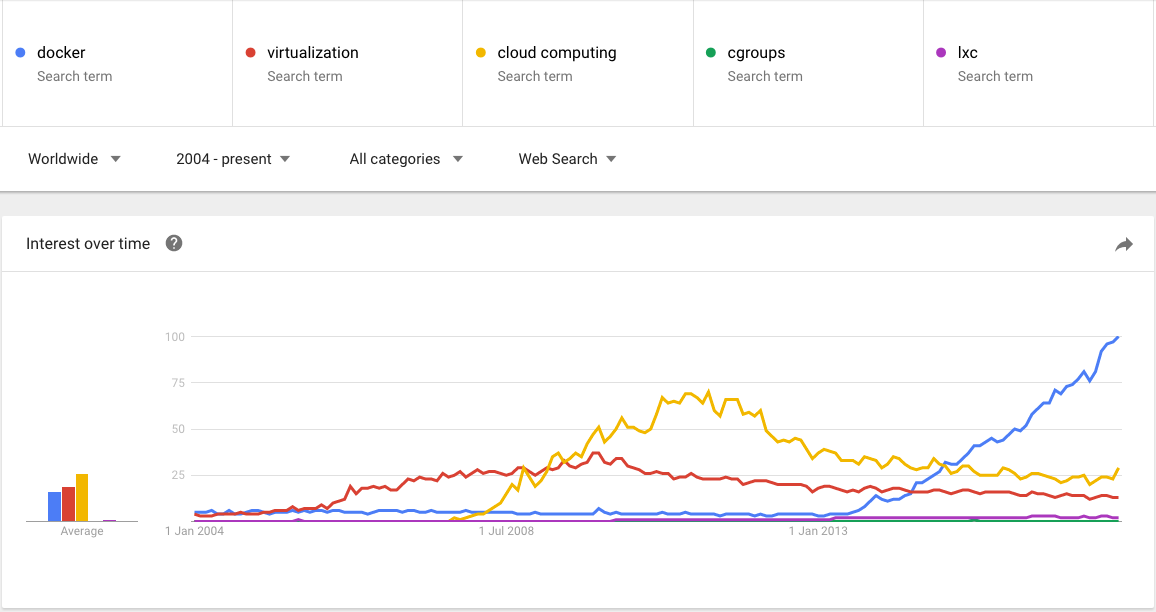
\includegraphics[width=13cm]{figure/trend}
    \caption{Google Trends of Container Technology (May 28, 2017)}
    \label{fig:trend}
\end{figure}

\skippara \cref{fig:arch} shows a high-level view of Docker's architecture
That is, the user uses (1) \gls{cli}-commands to interact with (2) Docker engine to manage Docker images, containers, network configurations, orchestration and more.
(3) containerd spins up container based on \gls{oci} container industry standard, such as (4) runc.
However, the fundamentals of container lie primarily around the Linux kernel features cgroups and namespaces.
In other words, cgroups ``limits how much you can use'' and namespaces ``limits what you can see (and therefore use)'' \cite{Anatomyo69:online}.

\begin{figure}[h!]
    \centering
    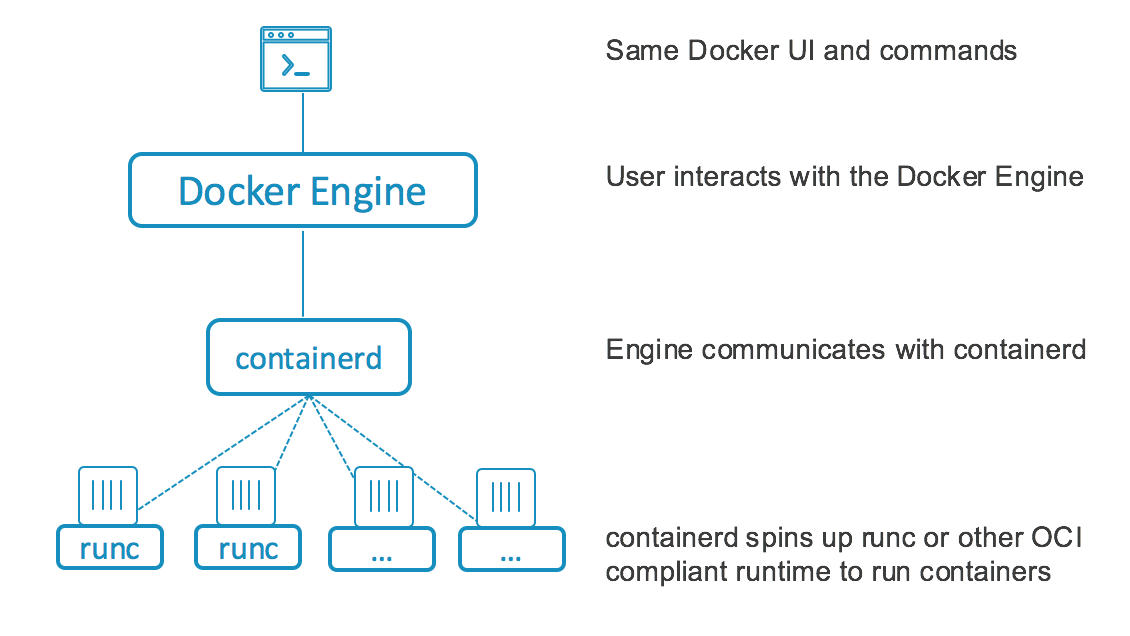
\includegraphics[width=11cm]{figure/dockerarchblog}
    \caption{Overview of Docker Architecture~\cite{Docker1199:online}}
    \label{fig:arch}
\end{figure}

\skippara Docker is feature rich in different ways to manage containers.
The following simplifies and describes a few Docker fundamentals.
That is, there are more advanced features that require specific \gls{cli}-flags to achieve a particular purpose.

\subsubsection{Docker Image}
Docker image is like a template, for example, a class in object-oriented programming.
An image contains different layers of the file system, for example, layer 1) Ubuntu base image and layer 2) updated packages.
Then, on top of all other layers, there is finally only a read-only file system layer.
It is possible to inspect the different layers of a Docker image with:
\begin{lstlisting}[numbers=none, frame=single]
  $ docker history <IMAGE_NAME:TAG>
\end{lstlisting}

\skippara There are two ways to create a Docker image. Either use already running container:
\begin{lstlisting}[numbers=none, frame=single]
  $ docker commit <RUNNING_CONTAINER> <IMAGE_NAME:TAG>
\end{lstlisting}

\skippara alternatively, build an image from a human-readable and portable file called Dockerfile:
\begin{lstlisting}[numbers=none, frame=single]
  $ docker build -t <IMAGE_NAME:TAG> <PATH_TO_DOCKERFILE_DIR>
\end{lstlisting}

\clearpage
\subsubsection{Docker Container}
Docker container is a running instance of an image, for example, an object in object-oriented programming.
Thus, once a container is running, it can then use the same hardware resources as the host kernel, such as file system, memory, \acrshort{cpu}, network, user and more.
For example:
\begin{lstlisting}[numbers=none, frame=single]
  $ docker run <IMAGE_NAME:TAG>
\end{lstlisting}

\skippara In our experiments, we followed the container technology standards to package the software in light-weight and portable containers.
It enabled us to move the software between environments with the dependencies intact more easily.
Also, the method to containerize the software facilitated the automation process of the tests.
